\documentclass[UTF8,a4paper,11pt,fontset=mac]{ctexart}
\usepackage[margin=22mm,top=24mm,bottom=23mm,headheight=14pt]{geometry}
\usepackage{amsmath,amssymb,booktabs,graphicx,caption,float,placeins}
\usepackage{siunitx,microtype,xcolor,fancyhdr,hyperref,array}
\hypersetup{colorlinks=true,linkcolor=black,urlcolor=blue!55!black,pdfauthor={TMD MLFF benchmark},pdftitle={三种 TMD 的 PBE 与 MLFF 声子及非线性耦合测试报告}}
\definecolor{ink}{HTML}{1C3549}
\definecolor{accent}{HTML}{1E618A}
\definecolor{light}{HTML}{EAF1F6}
\captionsetup{font=small,labelfont={bf,color=ink},skip=5pt}
\setlength{\parindent}{2em}
\setlength{\parskip}{2pt}
\setlength{\textfloatsep}{11pt plus 2pt minus 2pt}
\setlength{\floatsep}{9pt plus 2pt minus 2pt}
\setlength{\intextsep}{9pt plus 2pt minus 2pt}
\pagestyle{fancy}
\fancyhf{}
\fancyhead[L]{\small\color{ink}TMD 声子与非线性耦合定量测试}
\fancyhead[R]{\small\color{ink}GGA--PBE / MLFF}
\fancyfoot[C]{\thepage}
\renewcommand{\headrulewidth}{0.3pt}
\newcommand{\PhiC}{\Phi_{122}}
\newcommand{\PhiD}{\Phi_{1122}}
\newcommand{\Qunit}{\mathring{\mathrm A}\sqrt{\mathrm{amu}}}
\newcommand{\cubunit}{\mathrm{meV}/(\mathring{\mathrm A}^{3}\mathrm{amu}^{3/2})}
\newcommand{\quartunit}{\mathrm{meV}/(\mathring{\mathrm A}^{4}\mathrm{amu}^{2})}
\newcommand{\allwidthtable}[1]{\resizebox{\textwidth}{!}{\input{tables/#1.tex}}}
\newcommand{\figwide}[2]{\begin{figure}[!htbp]\centering\includegraphics[width=\textwidth]{figures/#1.pdf}\caption{#2}\label{fig:#1}\end{figure}}

\begin{document}
\begin{titlepage}
\color{ink}
\vspace*{27mm}
{\Large 静态声子与非线性势能面测试\par}
\vspace{8mm}
{\Huge\bfseries 三种二维 TMD 的 PBE--DFT 与机器学习力场对比\par}
\vspace{9mm}
{\Large WS$_2$、MoS$_2$、WSe$_2$；TECE / Prophet / EquiformerV3 + MatterSim\par}
\vspace{12mm}
\noindent\colorbox{light}{\parbox{0.94\textwidth}{\vspace{4mm}
\textbf{核心结论}\quad 将旧 PZ--LDA 参考换为重新弛豫的 GGA--PBE--USPP 后，三个材料五个通道的三阶耦合差距显著缩小；四阶耦合没有同步收敛。WS$_2$ 的 $\Gamma8$--M6 四阶变号在同一批原子构型和原始能量对比中仍然存在，因而不是绝对值排序或多项式拟合造成的。
\vspace{4mm}}}
\vfill
{\large 数据截至 2026 年 9 月 26 日\par}
\vspace{3mm}
{\normalsize 基于已完成的 6$\times$6 QE DFPT、579 个基线单点与 WS$_2$ 新增 208 个密网格单点\par}
\vspace{2mm}
{\small 独立研究报告；不含新的分子动力学与 Stage3 发布代码\par}
\end{titlepage}

\begin{abstract}
延续本科论文与此前测试报告的“声子谱及本征矢—模式对—二维势能面—非线性系数—数值可靠性—计算成本”分析顺序，本报告定量比较三种 1H 二维过渡金属二硫化物中 QE PZ--LDA、重新计算的 QE GGA--PBE、以及 TECE、Prophet、EquiformerV3 三条 Stage1 + MatterSim Stage2 路线。三种材料的 PBE 弛豫和 6$\times$6$\times$1 DFPT 均完成；各取原有筛选的五个 $\Gamma$--$q$--$(-q)$ 物理通道，计算中心 5$\times$5 高精度势能面，并对每种材料最强通道计算 9$\times$9 窗口。全部 579 个 QE 单点具有完整能量、原子力与来源校验。五通道三阶强度 $|\PhiC|$ 的 TECE+MatterSim 平均绝对误差从 LDA 参考的 10.33、12.54、3.94 降为 PBE 参考的 6.10、4.33、1.18 $\cubunit$；但 WS$_2$、MoS$_2$ 的四阶有符号误差略增。WS$_2$ $\Gamma8$--M6 在同一 PBE 结构、同一模式位移的 25 个构型上仍为 QE $-1.414$、MatterSim $+1.930$ $\quartunit$。新增的 WS$_2$ $\Gamma8$--M9 同构型 17$\times$17 位移网格表明：在固定宽窗口下，QE 四阶从 9$\times$9 到 17$\times$17 仅变动 $+0.152\%$，MatterSim 变动 $+4.917\%$；在固定中心窗口下分别变动 $+0.025\%$、$-0.392\%$。本结果支持以 PBE 参考开展后续筛选验证，同时要求对四阶物理量单独校准；不能用谐波频率精度替代高阶势能面验证。
\end{abstract}

\tableofcontents
\clearpage

\section{研究问题与比较范围}

本测试以原论文和此前稳定版的五个高耦合物理通道为固定比较对象，重点判断三个层次是否同时可信：第一，Stage1 的频率和本征矢能否识别相同声子对；第二，Stage2 给出的三、四阶耦合是否接近 DFT；第三，差异究竟源于参考泛函、模式映射、位移与拟合，还是势能面本身。原论文采用旧 PZ--LDA 超软赝势；MLFF 与其训练数据更接近的常见 GGA--PBE 参考不完全相同。因此本次重新以 PBE 弛豫晶胞和 PBE--USPP 计算三个材料，而不是只替换旧结构单点的泛函标签。

在三条 MLFF 路线中，Stage1 分别由 TECE、Prophet、EquiformerV3 在各自自行弛豫结构上经 Phonopy 得到谐波模式；Stage2 均使用同一 MatterSim 5M 权重计算非线性势能面。这样比较的是\emph{最终同一物理通道的系数}，而非把不同原子结构的绝对总能量相减。WS$_2$ $\Gamma8$--M6 另增加真正同构型的 25 点对照，用于诊断四阶变号。候选只包括 $\Gamma$ 光学模和有限 $q$ 的 $\Gamma$--$q$--$(-q)$ 耦合；$\Gamma$ 声学模不进入模式对。

这五对本来就是筛选出来的高强度通道，所以本报告的排序相关性仅在这五对内部定义，不代表所有候选的高通量召回率。本轮没有 SOC、非解析长程修正、旋转声学求和规则或分子动力学的验证。

\section{计算方法、单位与可比性}

\subsection{结构、DFPT 与模式匹配}

QE 7.4.1 使用标量相对论 PBE 超软赝势、$E_{\rm cut}^{\rm wfc}/E_{\rm cut}^{\rho}=120/1200$ Ry、原胞 $30\times30\times1$ $k$ 网格；三种二维晶胞均重新弛豫并满足设定收敛阈值。全 $6\times6\times1$ DFPT 数据经 \texttt{q2r} 与 \texttt{matdyn} 输出 36 个 $q$ 点的 9 支频率和本征矢。\texttt{simple} ASR 仅处理平移声学求和，不等于二维 ZA 所需的转动求和规则。频率统计除去 $\Gamma$ 点三支声学模，共 321 个值。

表~\ref{tab:geometry} 列出旧 LDA、新 PBE 与三条 MLFF 自行弛豫的面内晶格常数。新 PBE 比旧 LDA 大 1.73--2.19\%，而 MLFF 与 PBE 相差约 0.07--0.25\%。因此旧参考的几何压缩是此前差异的合理贡献之一，但表中变化同时包含交换相关和赝势族差别，无法单独分离几何作用。

\begin{table}[!htbp]\centering\small\caption{三种材料的自行弛豫面内晶格常数 $a$（Å）与 PBE 相对旧 LDA 的变化；E3 为 EquiformerV3。}\label{tab:geometry}
\begin{tabular}{lrrrrrr}
\toprule
材料 & 旧 LDA & 新 PBE & TECE & Prophet & E3 & PBE/LDA \\
\midrule
WS$_2$ & 3.1207 & 3.1881 & 3.1916 & 3.1923 & 3.1905 & 2.16\% \\
MoS$_2$ & 3.1290 & 3.1833 & 3.1898 & 3.1912 & 3.1882 & 1.73\% \\
WSe$_2$ & 3.2493 & 3.3204 & 3.3257 & 3.3267 & 3.3265 & 2.19\% \\
\bottomrule
\end{tabular}
\end{table}

模式对应由质量加权本征矢重叠 $|\langle e^{\rm PBE}_{q\nu},e^{X}_{q\mu}\rangle|^2$、频率和近简并子空间共同判定；不同计算的同一序号并不自动代表同一物理模。对于等价 $q$ 点，先按倒格矢和结构允许的操作对应，再比较模式；近简并单支的方向可随基底转动，故用子空间重叠解释，不能单独凭一个本征矢断言物理优劣。十五对关键通道的映射重叠平方最低为 0.99674（表~\ref{tab:mapping}）。

\begin{table}[!htbp]\centering\small
\caption{十五个固定物理通道的 PBE 频率与旧 LDA 至 PBE 的模式重叠。频率单位 THz。}\label{tab:mapping}
\allwidthtable{mode_mapping}
\end{table}

\subsection{二维实模势能面与导数}

统一使用质量归一化实模坐标 $Q$，单位为 $\Qunit$；从模式位移重建真实原子坐标，QE 和 MLFF 均求每个构型的总能量与原子力。对两个实模的能量差 $\Delta E=E(Q_1,Q_2)-E(0,0)$，中心 5$\times$5 网格（$Q_1,Q_2=-1,-0.5,0,0.5,1$）拟合 13 项多项式，设计矩阵满秩。报告的系数采用导数定义
\begin{equation}
\PhiC=\left.\frac{\partial^3 E}{\partial Q_1\partial Q_2^2}\right|_0,
\qquad
\PhiD=\left.\frac{\partial^4 E}{\partial Q_1^2\partial Q_2^2}\right|_0.
\label{eq:derivative}
\end{equation}
两者单位依次为 $\cubunit$、$\quartunit$。三阶排序使用 $|\PhiC|$，因为整体相位改变会翻转奇数次实模导数的符号；四阶保留\emph{有符号}的 $\PhiD$。最强通道的外层 9$\times$9 点使拟合窗口可扩展至 $|Q_i|\leq2$，与中心值比较，而不把宽窗外推值冒充局部 Taylor 导数。

参考值来自各自 PBE 模态坐标；MLFF 来自各自结构和模式。表中系数可比较同一物理通道的预测结果，但这本身不是同构型逐点 PES 误差。只有第~\ref{sec:same} 节的 WS$_2$ 检查同时固定了晶胞、原子顺序、模式位移与 25 个原子构型。

\subsection{误差、来源与数值门槛}

MAE/RMSE 在每种材料的五个固定通道上计算，三阶先取绝对值，四阶用有符号值。若旧档案缺标签则只按可恢复样本统计；WSe$_2$ 的旧 LDA 四阶只有一个标签，不能和新 PBE 五对误差作等样本前后比较。DFT 网格拟合前检查秩、残差、收敛与单位；18 点先导测试要求首通道三阶六点估计对 100$\to$120 Ry 和原胞等效 24$\to$30 $k$ 网格的变化均小于 2\%，之后才扩展完整网格。

\section{完整 $6\times6$ 声子谱与模式可靠性}

表~\ref{tab:phonons}、图~\ref{fig:phonon_summary}给出相对于新 PBE 的全网格误差。TECE 在三种材料上均为频率 MAE 最小的测试模型（0.065--0.093 THz），而 Prophet 的频率差通常更大（0.124--0.200 THz）；三者仍均明显小于旧 LDA 与 PBE 的差别。频率偏差显示 MLFF 对 PBE 多为系统性偏低，而旧 LDA 对 PBE 大多偏高。频率接近并不保证三、四阶导数接近。

\begin{table}[!htbp]\centering\small
\caption{相对于 QE PBE 的完整 $6\times6$ 频率比较。MAE、RMSE、偏差单位 THz；统计 321 个频率，排除 $\Gamma$ 声学三支。}\label{tab:phonons}
\allwidthtable{phonons}
\end{table}

\figwide{phonon_summary}{左：频率 MAE；右：近简并模式最差子空间重叠平方。WS$_2$ 中 Prophet 的近简并子空间指标最低，提示不能单看高重叠的孤立模。}

图~\ref{fig:qgrid_frequency_error}把每个 $q$ 点九个模式的匹配后平均绝对误差绘成 $6\times6$ 热图（$\Gamma$ 点只取光学六支）。热图能显示误差是否分布在整个网格，而不只集中于 M/K 等高对称点。三种材料中 Prophet 的误差偏大趋势具有网格范围，并非单个五对的特殊现象。

\begin{figure}[!htbp]\centering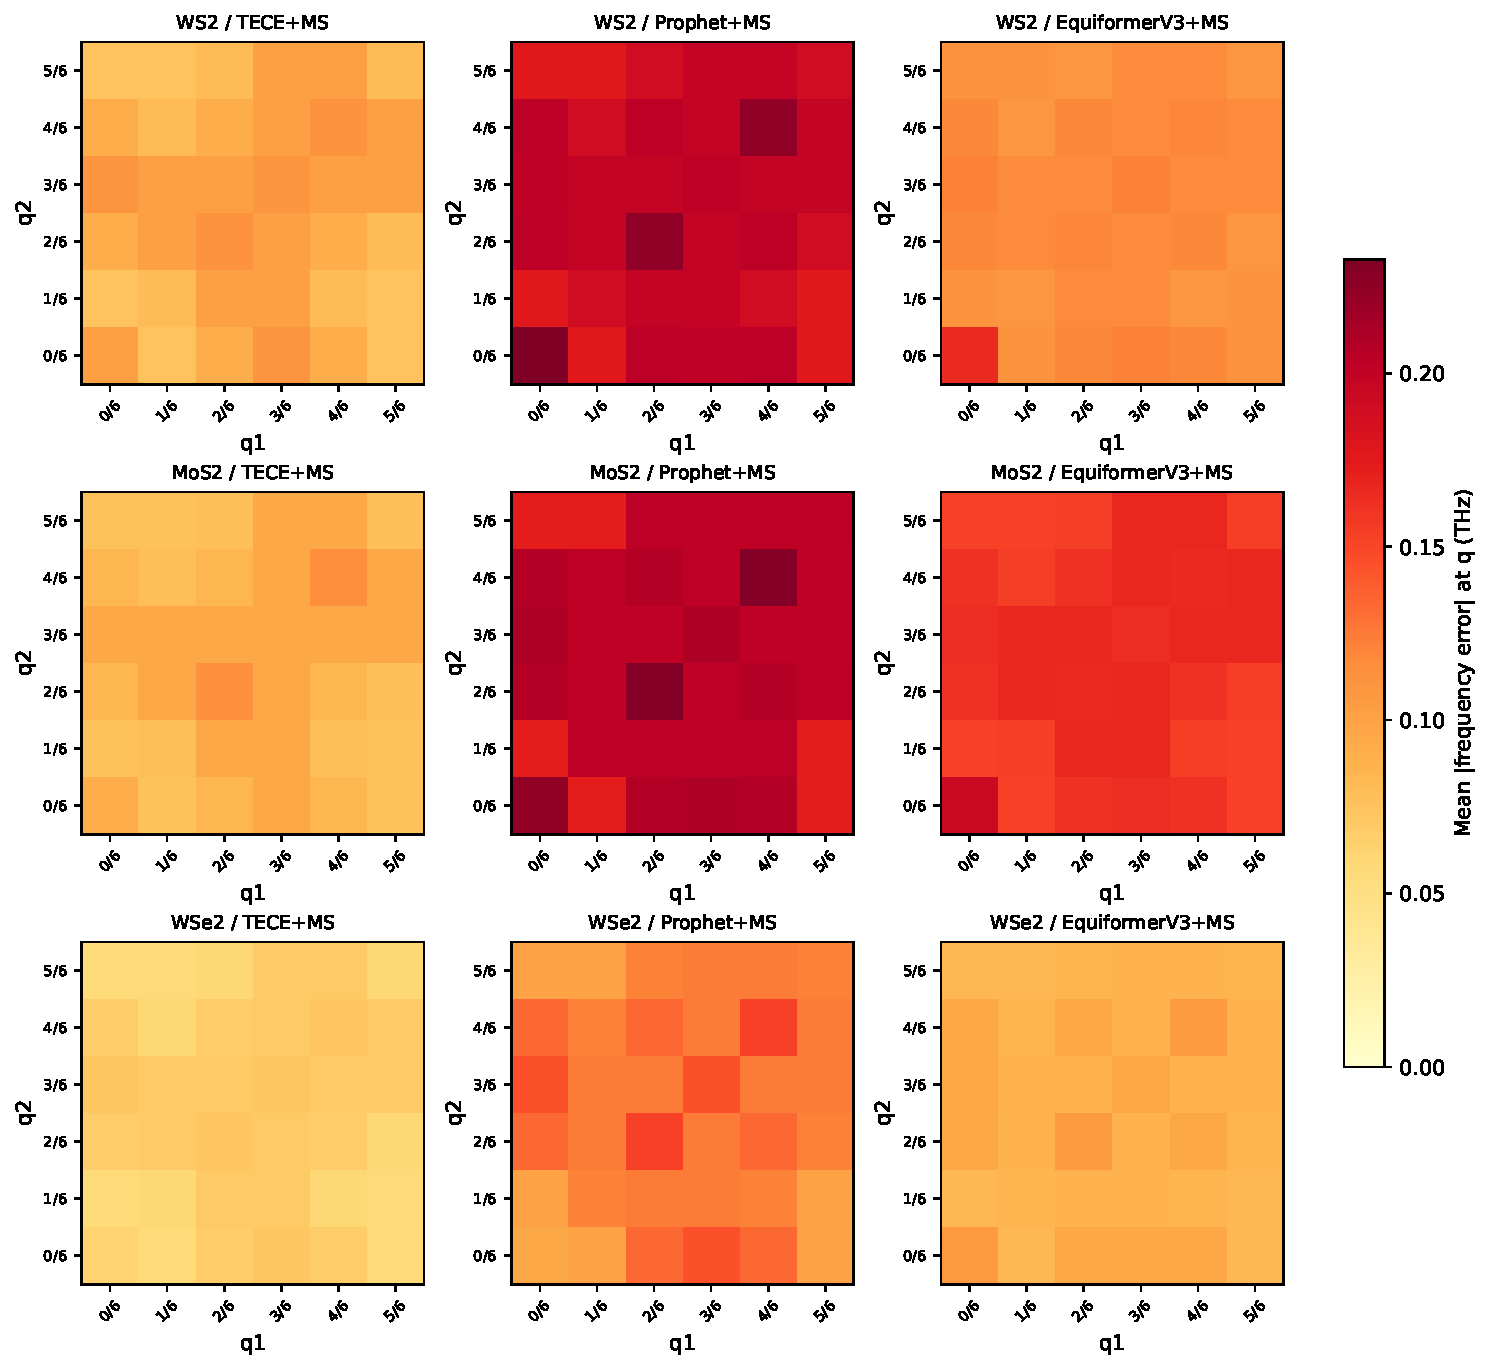
\includegraphics[width=0.88\textwidth]{figures/qgrid_frequency_error.pdf}
\caption{三种材料、三条 Stage1 路线的 $q$ 点平均频率绝对误差（THz）；同一颜色标尺，模式已按本征矢匹配。}\label{fig:qgrid_frequency_error}\end{figure}
\FloatBarrier

\section{三阶非线性耦合：参考泛函改变了多少}

表~\ref{tab:cubic-all} 与图~\ref{fig:cubic_channels}采用论文中逐模式对并列比较的形式，分别列出旧 LDA、新 PBE 与三条 MLFF 路线的五个 $|\PhiC|$。WS$_2$ 的 $\Gamma8$--M9 从旧 LDA 103.143 变为新 PBE 94.853，三条 MLFF 在 85.757--86.718；MoS$_2$ 同一通道从 106.134 降到 94.809，MLFF 在 88.725--89.423。参考改变明显缩小两者差距。WSe$_2$ 更接近，首通道 PBE 27.253、MLFF 25.945--26.152。

\begin{table}[!htbp]\centering\small
\caption{逐通道的三阶强度 $|\PhiC|$；单位 $\cubunit$。通道编号经本征矢匹配，而非直接按序号假定。}\label{tab:cubic-all}
\begin{minipage}{\textwidth}\centering\textbf{(a) WS$_2$}\par\allwidthtable{cubic_ws2}\vspace{3mm}
\textbf{(b) MoS$_2$}\par\allwidthtable{cubic_mos2}\vspace{3mm}
\textbf{(c) WSe$_2$}\par\allwidthtable{cubic_wse2}\end{minipage}
\end{table}

\begin{figure}[!htbp]\centering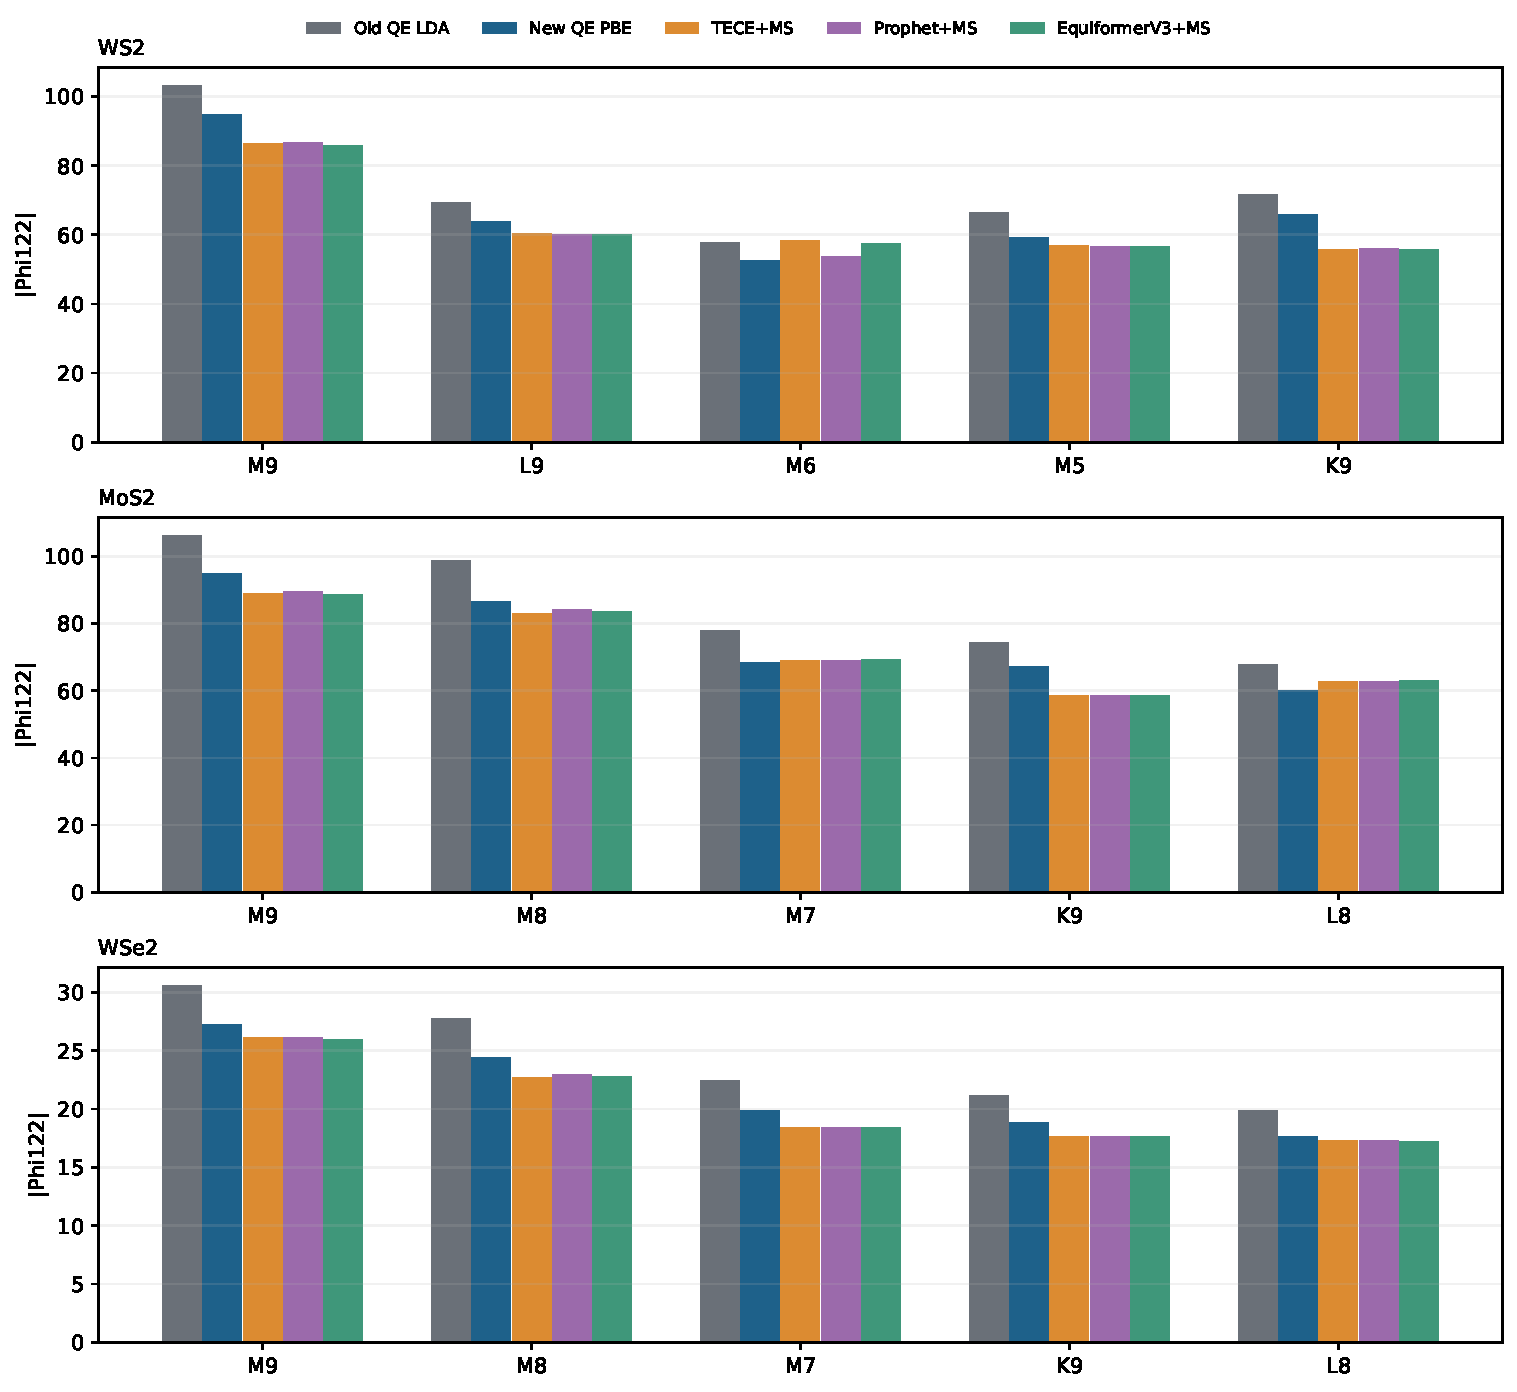
\includegraphics[width=0.92\textwidth]{figures/cubic_channels.pdf}
\caption{十五个固定通道的三阶强度并列比较；各材料五个通道分别排序展示。参考由 LDA 转至 PBE 后，首通道差距明显缩小。}\label{fig:cubic_channels}\end{figure}

量化结果见表~\ref{tab:metrics-pbe}、\ref{tab:metrics-lda}。TECE+MatterSim 的五对三阶 MAE 在 WS$_2$/MoS$_2$/WSe$_2$ 分别由旧 LDA 的 10.327/12.539/3.936 降为 PBE 的 6.104/4.328/1.180 $\cubunit$。Prophet+MatterSim 对 PBE 的三阶 MAE 在三材料均略低于 TECE，但三种模型间差异小于 DFT 参考切换的效应；这主要比较了不同 Stage1 模式/结构在同一 MatterSim Stage2 下的最终结果，不能据此推出 Prophet 谐波频率更准。

\begin{table}[!htbp]\centering\small
\caption{MLFF 对新 PBE 的误差。$n_3,n_4$ 为可比较通道数，三、四阶单位分别见式~\eqref{eq:derivative}。}\label{tab:metrics-pbe}
\allwidthtable{metrics_pbe}
\end{table}
\begin{table}[!htbp]\centering\small
\caption{同样的 MLFF 结果对旧 LDA 的误差。WSe$_2$ 旧四阶仅 $n_4=1$，不可与新参考的五对误差直接比较。}\label{tab:metrics-lda}
\allwidthtable{metrics_lda}
\end{table}
\FloatBarrier

\section{四阶耦合、排序与关键异常}

表~\ref{tab:quartic-all} 与图~\ref{fig:quartic_channels}保留四阶导数的符号。最突出的 WS$_2$ $\Gamma8$--M6：旧 LDA 为 $-1.533$，新 PBE 为 $-1.414$，但三条自行弛豫的 MatterSim 路线均为 $+1.89$ 至 $+1.93$ $\quartunit$。WS$_2$ 与 MoS$_2$ 的五对四阶 MAE 在 PBE 参考下未下降；因此三阶改进不能延伸为“高阶势能面已整体准确”。WSe$_2$ 新 PBE 四阶五对有结果、TECE+MatterSim MAE 为 0.628，但旧数据只支持一对，不作改善百分比声明。

\begin{table}[!htbp]\centering\small
\caption{逐通道有符号四阶 $\PhiD$，单位 $\quartunit$；破折号表示旧档案没有可用标签。}\label{tab:quartic-all}
\begin{minipage}{\textwidth}\centering\textbf{(a) WS$_2$}\par\allwidthtable{quartic_ws2}\vspace{3mm}
\textbf{(b) MoS$_2$}\par\allwidthtable{quartic_mos2}\vspace{3mm}
\textbf{(c) WSe$_2$}\par\allwidthtable{quartic_wse2}\end{minipage}
\end{table}

\begin{figure}[!htbp]\centering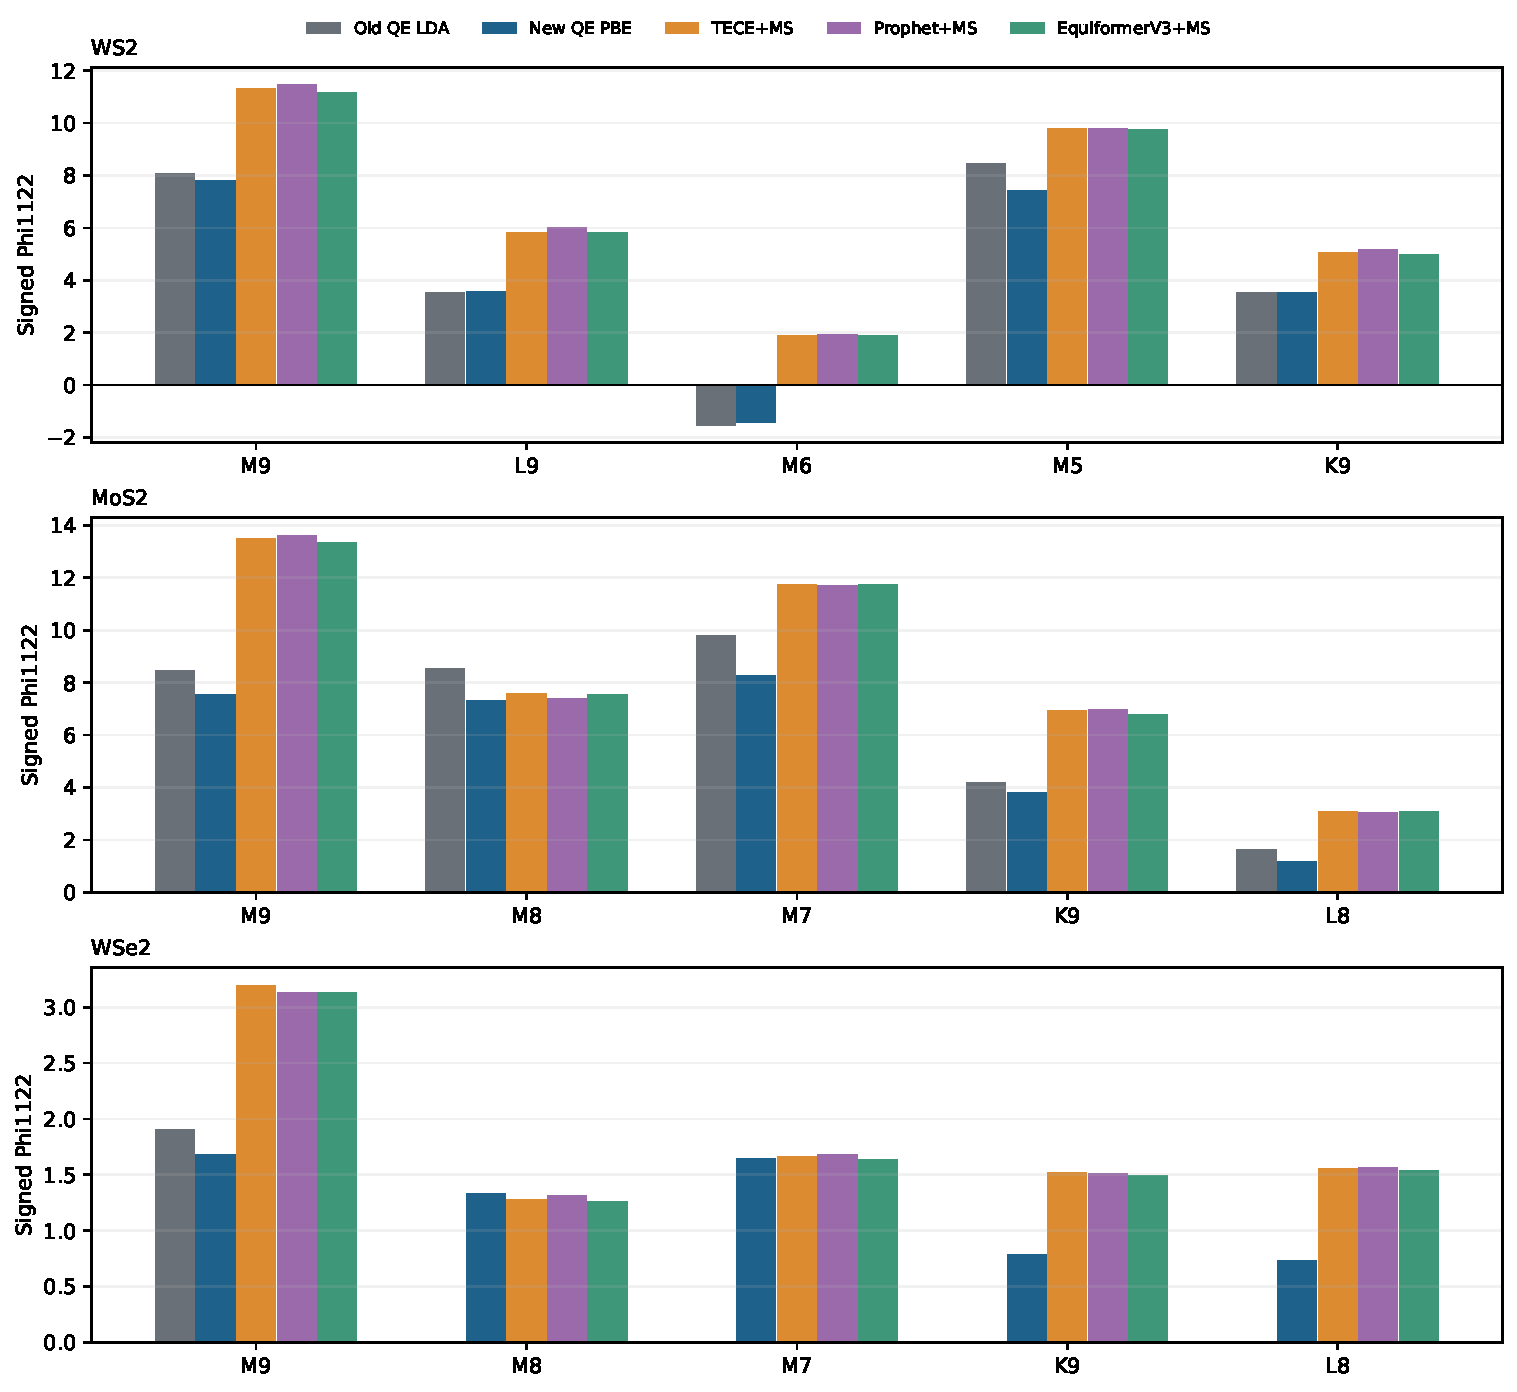
\includegraphics[width=0.92\textwidth]{figures/quartic_channels.pdf}
\caption{有符号四阶导数对比；WS$_2$ 的 M6 通道显示参考和 MLFF 势能面的实质性变号。}\label{fig:quartic_channels}\end{figure}

图~\ref{fig:coupling_scatter}将 45 个“材料--通道--Stage1 路线”点与 PBE 比较。三阶散点总体沿对角线，但较强通道多被 MLFF 低估；四阶散点的系统性上移和 WS$_2$ M6 变号同时可见。三个 Stage1 的散点彼此紧邻，表明目前仅更换 Stage1 对四阶偏差的改善有限；这也是后续需要考虑 Stage2 校准的依据。

\figwide{coupling_scatter}{三阶强度（左）与有符号四阶（右）相对 PBE 的散点。每种材料五对、每对三条 Stage1 路线；虚线为完全一致。}

在五对内部，$|\PhiC|$ 的 Spearman 排名相关系数见表~\ref{tab:rank}。MoS$_2$ 的三条路线均为 0.90，WSe$_2$ 均为 1.00；WS$_2$ 的 TECE/EquiformerV3 为 0.30，Prophet 为 0.70。该指标描述\emph{已选五对}内部的排序稳定性，不能替代全候选粗筛的遗漏率。

\begin{table}[!htbp]\centering\small\caption{五对已选通道内部 $|\PhiC|$ 排名对 PBE 的 Spearman 系数。}\label{tab:rank}
\begin{tabular}{lrrr}
\toprule
材料 & TECE+MS & Prophet+MS & EquiformerV3+MS \\
\midrule
WS$_2$ & 0.30 & 0.70 & 0.30 \\
MoS$_2$ & 0.90 & 0.90 & 0.90 \\
WSe$_2$ & 1.00 & 1.00 & 1.00 \\
\bottomrule
\end{tabular}
\end{table}
\FloatBarrier

\section{WS$_2$ 同构型势能面：四阶符号差异的来源}\label{sec:same}

为了将“参考不同”“模式位移不同”“拟合定义不同”区分开，直接使用 PBE QE $\Gamma8$--M6 的 25 个原始输入结构，保持晶胞、元素、顺序、位置与两个质量归一化实模坐标相同，再用 MatterSim 5M 评价。检查的最大周期位置偏差小于 $10^{-6}$ Å。两方法分别减去各自 $Q_1=Q_2=0$ 的能量，避免不相容绝对总能量的比较。两组 13 项拟合 RMSE 分别只有 0.01123 和 0.01453 meV/超胞，而四阶结果为 QE $-1.414104$、MatterSim $+1.930393$ $\quartunit$。

更关键的是不依赖多项式拟合的偶混合能量差：
\begin{equation}
\Delta E_{\rm even}(Q)=\frac14\sum_{s,t=\pm1}E(sQ,tQ)
-\frac12\sum_{s=\pm1}E(sQ,0)
-\frac12\sum_{t=\pm1}E(0,tQ)+E(0,0).
\label{eq:even}
\end{equation}
它抵消两个纯轴项及奇混合项；局部四阶主导时 $4\Delta E_{\rm even}/Q^4\approx\PhiD$。在 $Q=0.5$、1，两种方法的原始能量差符号相反（表~\ref{tab:m6}），且两点给出的有效四阶几乎相同。这排除了\emph{单纯}的绝对值排名、模态相位及 13 项拟合算法导致的符号反转。QE PBE--USPP 与 MatterSim 训练标签仍可能不同，结果只针对这个已固定的参考协议。

\begin{table}[!htbp]\centering\small\caption{WS$_2$ M6 同构型原始偶混合差。$Q$ 单位 $\Qunit$，$\Delta E$ 单位 meV/超胞，最后两列单位 $\quartunit$。}\label{tab:m6}
\begin{tabular}{lrrrr}
\toprule
$Q$ & PBE $\Delta E$ & MS $\Delta E$ & PBE $4\Delta E/Q^4$ & MS $4\Delta E/Q^4$ \\
\midrule
0.5 & -0.02184 & 0.03052 & -1.398 & 1.953 \\
1.0 & -0.35252 & 0.49472 & -1.410 & 1.979 \\
\bottomrule
\end{tabular}
\end{table}
\begin{figure}[!htbp]\centering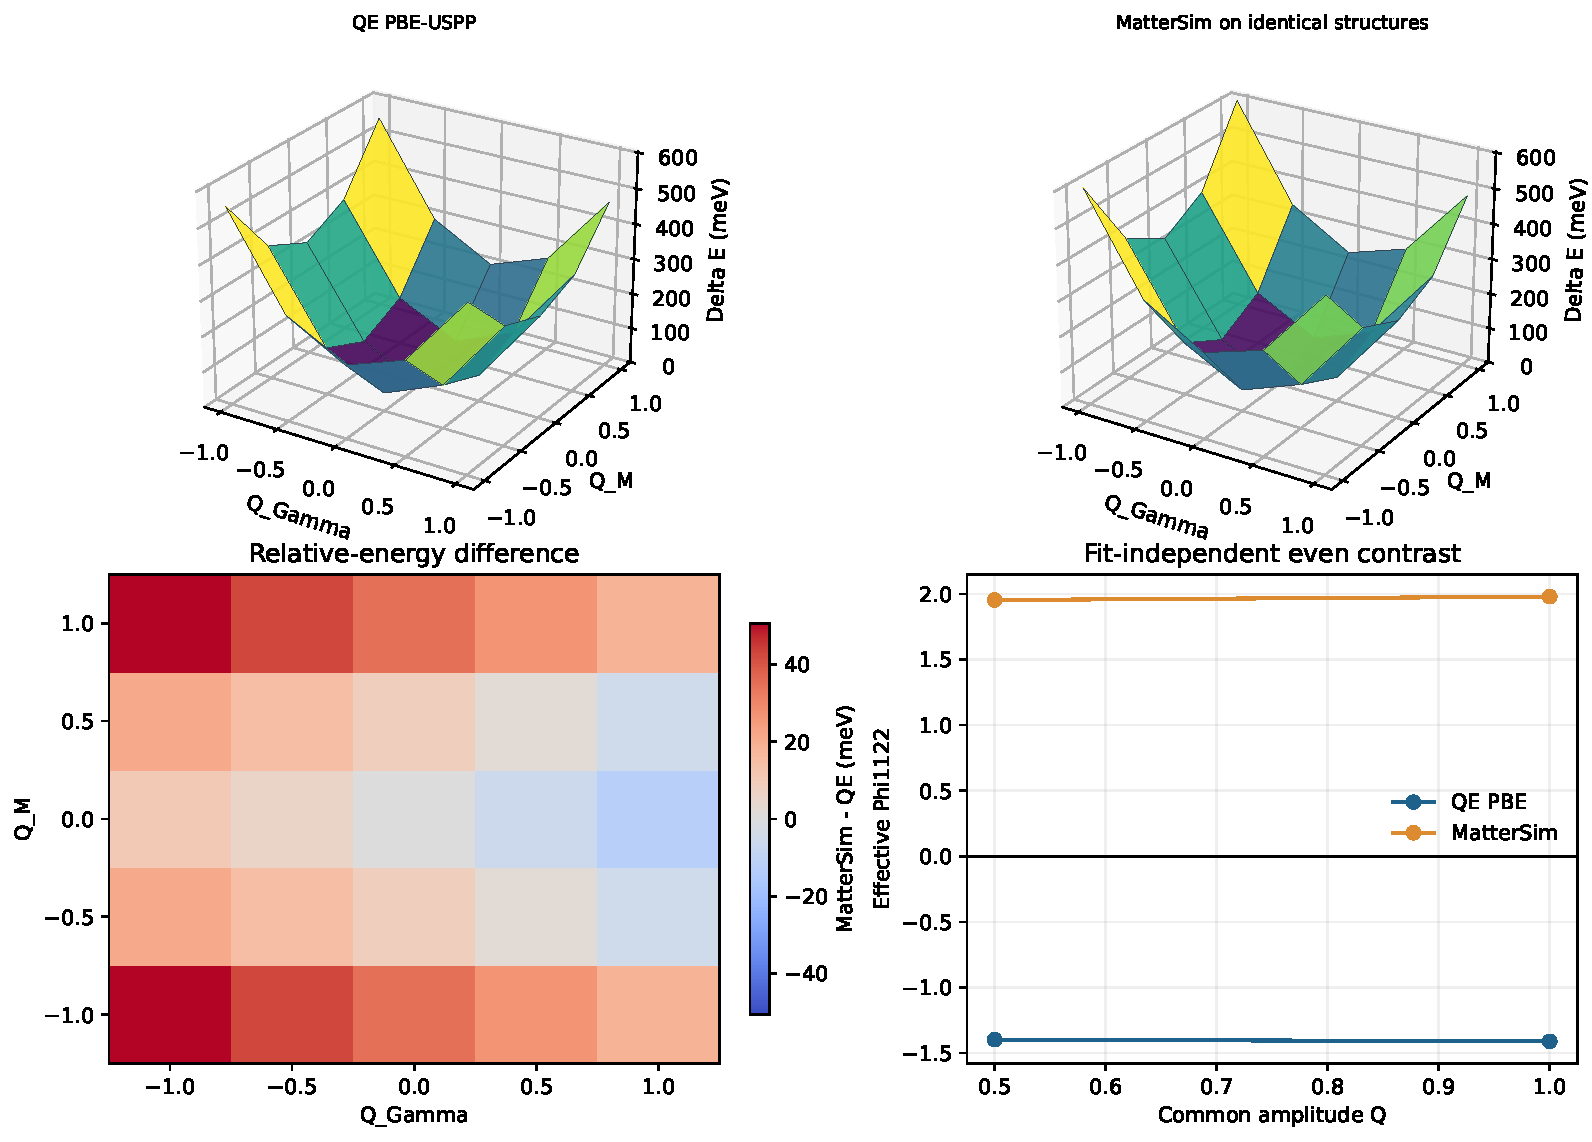
\includegraphics[width=0.93\textwidth]{figures/ws2_m6_same_geometry_pes.pdf}
\caption{WS$_2$ M6 在相同 25 个构型上的 QE PBE 与 MatterSim 二维势能面、相对能差及拟合无关的偶混合对比。三维曲面的总体相似并不能保证微小四阶混合项同号。}\label{fig:ws2_m6_same_geometry_pes}\end{figure}

在相同构型上，相对能量的 MAE 为 19.404 meV/超胞，RMSE 为 24.629 meV/超胞。900 个笛卡尔力分量的 MAE 为 0.02856 eV/Å，RMSE 为 0.05486 eV/Å（图~\ref{fig:ws2_m6_pointwise_errors}）。此处才能严格称为同构型能量和力误差。两组全局曲率都使曲面呈碗状，但低能量尺度的交叉四阶项显著不同，说明能量或力总体相关性不能代替目标耦合项的检测。

\figwide{ws2_m6_pointwise_errors}{同一 25 个 WS$_2$ PBE 构型的相对能量、900 个力分量及逐点相对能量差；仅此对照固定了所有原子坐标。}
\FloatBarrier

\section{拟合质量、窗口与电子收敛}

表~\ref{tab:fit} 和图~\ref{fig:fit_residual_window}给出中心 5$\times$5 网格的残差。所有十五个 QE 网格的设计矩阵均为秩 13；残差一般远小于势能面变化，但残差低本身不保证导数无系统偏差。对于任意非零有限 $q$，$\Gamma$--$\Gamma$--$q$ 在理想无限晶体均不满足动量守恒，故 $\Phi_{112}$ 的拟合值应作为数值诊断而非允许的物理耦合。L/K 点的可见小残值须进一步检查超胞、离散网格或拟合误差，不能以“L 点例外”解释。

\begin{table}[!htbp]\centering\small\caption{中心 5$\times$5 多项式拟合诊断。RMSE 单位 meV/超胞；末列 $|\Phi_{112}|$ 单位 $\cubunit$。TECE/Prophet/E3 列均为同一 MatterSim Stage2，但使用各自模式。}\label{tab:fit}
\allwidthtable{fit_diagnostics}\end{table}

\figwide{fit_residual_window}{左：每个通道中心拟合残差；右：每材料最强通道四阶值随窗口扩大而变化。低残差与低窗口敏感性是不同的检验。}

最强通道的 PBE 四阶中心值到 $|Q|\leq2$ 的变化分别为 WS$_2$ $-1.39\%$、MoS$_2$ $-1.76\%$、WSe$_2$ $+0.25\%$（表~\ref{tab:window}）；这支持这三个首通道在当前窗口内相对稳定，\emph{不能外推到其余十二对}。WS$_2$ M6 的 $Q=0.5$ 与 1 的式~\eqref{eq:even} 对比为该异常另提供两尺度检验。

计算的来源检查覆盖 579/579 个不同作业：输入、脚本、输出哈希匹配，QE 能量与原子力齐全，程序正常退出。显式 \texttt{input\_dft='PBE'} 与从 UPF 推断 PBE 的交叉检查得到逐项相同的能量和力。先导门槛仅验证首通道三阶对截止能和 $k$ 网格的稳定性，不是全部四阶项的严格电子收敛证明。报告仍以 PBE--USPP 为内部统一 DFT 参考，而不宣称复现 MatterSim 的原始训练标签。

\begin{table}[!htbp]\centering\small\caption{每材料最强通道 PBE $\PhiD$ 的 5$\times$5、7$\times$7、9$\times$9 拟合窗口敏感性；RMSE 单位 meV/超胞。}\label{tab:window}
\begin{tabular}{lrrrrr}
\toprule
材料 & $|Q|\leq1$ & $|Q|\leq1.5$ & $|Q|\leq2$ & 中心到宽窗 & 宽窗 RMSE \\
\midrule
WS$_2$ & 7.798 & 7.755 & 7.690 & -1.39\% & 0.0759 \\
MoS$_2$ & 7.557 & 7.501 & 7.424 & -1.76\% & 0.0374 \\
WSe$_2$ & 1.680 & 1.681 & 1.684 & +0.25\% & 0.0189 \\
\bottomrule
\end{tabular}
\end{table}

\subsection{固定窗口的位移采样密度核查（补充）}

这里的 $6\times6$ 是\emph{倒空间声子 $q$ 网格}，不是二维势能面的位移网格。原先表~\ref{tab:window} 从 5$\times$5 的 $|Q_i|\leq1$ 到 9$\times$9 的 $|Q_i|\leq2$，步长均为 0.5 $\Qunit$；它检验的是\emph{拟合窗口}，不能单独称为网格密度收敛。为纠正这一点，重新抽取每个材料最强通道已经完成的 81 个 QE 点，在完全相同的 $|Q_i|\leq2$ 范围内比较稀疏 5$\times$5（步长 1.0）与密集 9$\times$9（步长 0.5），均用同一 13 项拟合器且秩为 13。密度加倍引起的四阶变化依次为 WS$_2$ $+0.168\%$、MoS$_2$ $+0.199\%$、WSe$_2$ $-0.029\%$（表~\ref{tab:density}，图~\ref{fig:displacement_density}）。

\begin{table}[!htbp]\centering\small\caption{每材料最强通道的有符号 PBE $\PhiD$ 位移密度复核，单位 $\quartunit$。中心 5$\times$5 的窗口为 $|Q_i|\leq1$、步长 0.5；后两列固定 $|Q_i|\leq2$，分别取步长 1.0 和 0.5。百分比仅比较后两列。}\label{tab:density}
\allwidthtable{density}\end{table}

\begin{figure}[!htbp]\centering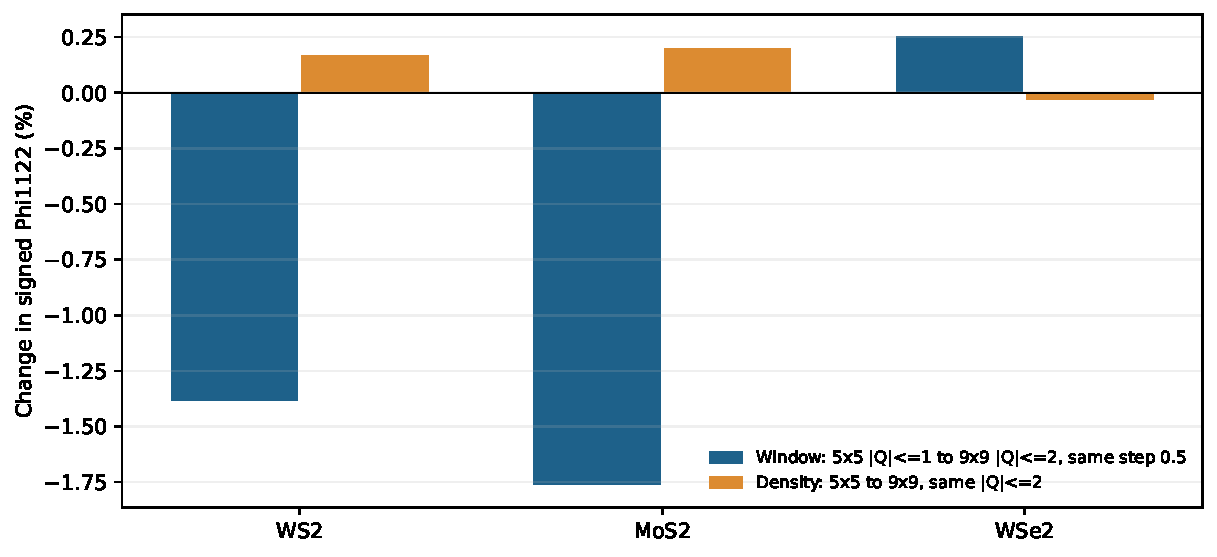
\includegraphics[width=0.82\textwidth]{figures/displacement_density.pdf}
\caption{将窗口变化与固定窗口下的采样密度变化分开展示。蓝色包含 $|Q|\leq1\to2$ 的窗口效应；橙色只改变 $|Q|\leq2$ 内的步长。}\label{fig:displacement_density}\end{figure}

这说明\emph{三个最强通道在原有宽窗口数据内}对第一次密度加倍不敏感；尚不足以证明局部四阶 Taylor 导数已严格收敛。原档案中其他十二对只有中心 5$\times$5，中心 $|Q_i|\leq1$ 的 9$\times$9（步长 0.25）当时未计算。以下新增 WS$_2$ 首通道的密网格，不能替代 MoS$_2$、WSe$_2$ 或 WS$_2$ M6 的同类检验。WS$_2$ M6 的 $Q=0.5$、1 偶混合对比确认变号不是单个步长或拟合算法产生，但仍需要该通道的固定窗口密度测试。

\subsection{新增 WS$_2$ 首通道 17$\times$17 同构型密网格}

另对 WS$_2$ $\Gamma8$--M9 在\emph{相同} $|Q_\Gamma|,|Q_q|\leq2\,\Qunit$ 上计算嵌套 17$\times$17 网格，步长从 0.5 减为 0.25。旧 9$\times$9 的 81 个 QE 点逐一核对结构及输入、输出哈希后复用；新增 208 个 QE PBE--USPP 单点均收敛并有全部 12 个原子力。MatterSim 5M 在\emph{完全相同}的 289 个原子构型上计算。这是首通道的额外密度实验，不改变其余十四通道的已有计算。

表~\ref{tab:densews2} 同时给出固定宽窗 $|Q|\leq2$ 和固定中心窗 $|Q|\leq1$ 的三、四阶结果。宽窗 9$\times$9 $\to$ 17$\times$17 时，QE 的有符号 $\PhiD$ 为 $7.6905\to7.7022\,\quartunit$（$+0.152\%$），MatterSim 为 $8.0011\to8.3945\,\quartunit$（$+4.917\%$）。同一宽窗内 QE 的 $|\PhiC|$ 为 $94.7903\to94.7967\,\cubunit$，MatterSim 为 $87.2202\to87.4178\,\cubunit$。该通道宽窗四阶拟合对加密的敏感性主要发生在 MatterSim 一侧。

中心窗 5$\times$5 $\to$ 9$\times$9 时，QE 的 $\PhiD$ 为 $7.7985\to7.8005$（$+0.025\%$），MatterSim 为 $11.2105\to11.1666$（$-0.392\%$），两者仍相差 $3.3661\,\quartunit$。在更小的 $|Q|\leq0.5$ 窗口，QE/MatterSim 分别为 $7.8042/11.3401\,\quartunit$。把\emph{宽窗}与\emph{中心窗}互相比会混入窗口效应，不能误称为采样密度收敛。

13 项拟合在宽窗 9$\times$9/17$\times$17 上的 QE 残差 RMSE 为 $0.0759/0.0654$ meV/超胞，MatterSim 为 $0.8877/0.7097$ meV/超胞；中心窗 5$\times$5/9$\times$9 则分别为 QE $0.00269/0.00250$、MatterSim $0.1144/0.0982$ meV/超胞。因而这里的“密度变化”严格指\emph{同一 13 项有限窗口拟合在加密取样后的稳定性}，不能直接等同于解析势能面的零位移四阶 Taylor 导数。MatterSim 的宽窗残差较大，提示有限窗口内还有该多项式未充分描述的形状或数值误差。

\begin{table}[!htbp]\centering\small
\caption{WS$_2$ $\Gamma8$--M9 相同构型的固定窗口密度对照。$\Delta Q$ 单位 $\Qunit$；三、四阶单位分别为 $\cubunit$、$\quartunit$；相对中心点能量 MAE 为 meV/超胞，力分量 MAE 为 eV/Å。各拟合设计矩阵秩为 13。}
\label{tab:densews2}
\allwidthtable{dense_ws2}
\end{table}
本次检查覆盖 208 个新点与 81 个复用点的无重复索引、完整原子力、旧 5$\times$5/9$\times$9 系数复现、相同模式坐标和结构哈希。结论只针对\emph{一个首通道}；不能推出另外十四通道或 WS$_2$ M6 变号已经完成同等级别的密度收敛检验。

\figwide{dense_ws2}{固定宽窗（左）与中心窗（右）内，QE PBE 和同构型 MatterSim 的有符号四阶系数随位移采样步长变化。}

289 个同构型点上，相对中心能量 MAE/RMSE 为 $10.072/12.036$ meV/超胞，10404 个力分量的 MAE/RMSE 为 $0.02136/0.04047$ eV/Å；中心 $|Q|\leq1$ 的 81 点分别为 $5.834/6.923$ meV/超胞和 $0.01145/0.01917$ eV/Å。低总能量或力误差并不确保目标四阶系数接近。式~\eqref{eq:even} 的偶混合原始能量差也分别在两套 289 点上直接计算：QE 的等幅有效 $\PhiD$ 在 $Q=0.25,0.5,1,2$ 处约为 $7.77,7.79,7.80,7.69$，MatterSim 为 $13.67,11.06,11.18,8.17\,\quartunit$（图~\ref{fig:dense_ws2_even_mixed}）。MatterSim 的 $Q=0.25$ 项对微小能量差及浮点精度特别敏感，不宜单点外推为 Taylor 导数；但 $Q=0.5$ 和 1 的差异直接见于原始能量组合。
\figwide{dense_ws2_even_mixed}{不经过多项式拟合，由等幅四角点和坐标轴能量直接计算的有符号偶混合四阶估计。最小振幅的 MatterSim 值对浮点精度敏感。}


\FloatBarrier

\begin{table}[!htbp]\centering\small\caption{三种材料的首通道 18 点电子收敛先导结果：六点三阶估计的相对变化，均满足预设 2\% 停机门槛。}\label{tab:pilots}
\begin{tabular}{lrrr}
\toprule
材料 & 100$\to$120 Ry & 24$\to$30 $k$ 网格 & 2\% 门槛 \\
\midrule
WS$_2$ & 0.0051\% & 0.00014\% & 通过 \\
MoS$_2$ & 0.0051\% & 0.00014\% & 通过 \\
WSe$_2$ & 0.0469\% & 0.00050\% & 通过 \\
\bottomrule
\end{tabular}
\end{table}

\FloatBarrier

\section{成本、适用性与下一轮实验}

三个材料的基线实验分别完成 193 个 QE 单点：五对中心 25 点、最强对补齐 81 点，以及先导点，总计 579 点。按 Slurm 计量，这 579 个 PBE 势能面单点合计 104.09 节点时；该数不包括新增 WS$_2$ 密网格的 208 个单点、三次 DFPT、控制器或 MLFF 早期筛选。新增 208 个 QE 点按 Slurm 实际计量为 21.059 节点时；另一次因节点过载而取消的尝试耗费约 0.300 节点时，均不含控制器和已复用的 81 点。12 原子的 M/K 模式单点中位数约 5.8--6.7 分钟，27 原子的 L 模式约 22--27 分钟（表~\ref{tab:cost}；图~\ref{fig:compute_cost}）。因此先以便宜的 MLFF 在所有候选上排序、仅对强耦合且可信的模式做 DFT，是有实际计算意义的；本报告没有测定本轮各 Stage1/Stage2 的完整端到端墙钟，不能从此表推算 MLFF 的精确加速比。

\begin{table}[!htbp]\centering\small\caption{QE PBE PES 单点的实际 Slurm 成本。节点时按单点作业计，不含 DFPT 与控制器；中位秒按相应原子数分组。}\label{tab:cost}
\begin{tabular}{lrrrr}
\toprule
材料 & QE 单点 & 12 原子中位秒 & 27 原子中位秒 & 节点时 \\
\midrule
WS$_2$ & 193 & 367.4 & 1429.2 & 34.36 \\
MoS$_2$ & 193 & 345.8 & 1312.9 & 31.08 \\
WSe$_2$ & 193 & 403.7 & 1643.9 & 38.65 \\
\bottomrule
\end{tabular}
\end{table}
\figwide{compute_cost}{左：12 与 27 原子超胞的 QE 单点中位墙钟；右：各材料 193 个单点的累计节点时。}

\noindent\textbf{方法学结论。} 以 TECE/Prophet/EquiformerV3 进行 Stage1、MatterSim 做 Stage2 的筛选路线在谐波模式识别和五对三阶强度上有用；PBE 参考比旧 LDA 更适合本轮数值对照。但三种 Stage1 更换后，某些四阶偏差仍共同存在，WS$_2$ M6 在完全相同输入上证实存在 PES 差异。因此下一轮优先级是：在统一 PBE--USPP 标签与相同几何上，对可疑的四阶通道做少量 DFT 校准；用保留的混合偶差和窗口敏感性作为主动选点指标；然后才评估不同 Stage2 或知识蒸馏是否保留这些高阶导数。扩大材料和候选数时，必须同时报告全候选粗筛召回率，而不仅是当前前五名内部相关系数。

\noindent\textbf{解释边界。} 从 LDA 到 PBE 同时更换交换相关近似、赝势族和弛豫结构，不能把三阶 MAE 下降单独归因于泛函。MLFF 路线使用自行弛豫的各自模式；只有专门的 WS$_2$ M6 测试严格比较同构型能量与力。平移 ASR 不确保 ZA 的二维转动约束。所有结果限于静态局域 PES，不能直接证明长时间 MD 的稳定性或动力学性质。

\clearpage
\appendix
\section{可追溯材料与复现}

本报告的所有数字、表格和图由同一套机器可读结果直接生成。原始 PBE 点位于独立研究归档，主要综合文件为：
\begin{itemize}\setlength{\itemsep}{0pt}
\item \texttt{coupling\_comparison.json}、三个 \texttt{results\_*.json}；
\item 三个 \texttt{*\_phonon\_comparison.json}、\texttt{structure\_comparison.json}；
\item \texttt{campaign\_audit.json}、\texttt{ws2\_pbe\_geometry\_mattersim\_m6.json}；
\item 新增密网格的 \texttt{docs/reference\_data/pbe\_20260925/ws2\_17x17\_qe.json}、\texttt{ws2\_17x17\_mattersim.json} 与 \texttt{ws2\_17x17\_resource\_audit.json}，包含 289 点能量和力、拟合、偶混合检验及 208 个新点的 Slurm 资源记录。
\end{itemize}
旧模型参考只读取 Git 稳定仓库的验收数据目录，没有修改稳定代码。基线报表输入文件的 SHA256 保存在本目录的 \texttt{sources.json}；新增 WS$_2$ 密网格输入哈希见 \texttt{dense\_ws2\_sources.json}。运行 \texttt{generate\_assets.py} 可重建图表，随后用 XeLaTeX 编译本文件。主比较按五对物理通道对应，旧 WSe$_2$ 未恢复的四阶值如实显示为缺失。

\begin{thebibliography}{9}
\bibitem{thesis} 本科毕业论文（最终版），第 3--4 章：声子模式、二维势能面与非线性耦合的报告形式及旧 DFT 结果。
\bibitem{prior} \texttt{model\_dft\_comparison\_1\_0\_1.pdf}、\texttt{hex\_phonopy\_acceptance\_1\_0\_1.pdf} 与 WS$_2$ top5 DFT 比较报告：此前的测试口径、模式对与图表顺序。
\bibitem{campaign} PBE 三材料独立研究归档（2026-09-25 至 2026-09-26）：QE 输入输出、Slurm 记录、哈希审计、全网格声子与同构型 WS$_2$ 势能面。
\end{thebibliography}

\end{document}
